\documentclass[conference]{IEEEtran}
\IEEEoverridecommandlockouts
% The preceding line is only needed to identify funding in the first footnote. If that is unneeded, please comment it out.
\usepackage{cite}
\usepackage{amsmath,amssymb,amsfonts}
\usepackage{algorithmic}
\usepackage{graphicx}
\usepackage{textcomp}
\usepackage{xcolor}
% preamble additions
\usepackage{booktabs}
\usepackage{url}
\def\BibTeX{{\rm B\kern-.05em{\sc i\kern-.025em b}\kern-.08em
    T\kern-.1667em\lower.7ex\hbox{E}\kern-.125emX}}
\begin{document}

\title{University of Pretoria \\MIT 805 Group 19\\Group Project Part 2\\}

\author{\IEEEauthorblockN{Shreya Bharat \\19031786}
\and
\IEEEauthorblockN{Lerato Mokori\\26834694}}


\maketitle
\section{Introduction}
The TLC Trip Record Dataset contains data collected by the NYC Taxi and Limousine Commission (TLC) on taxi trip records, including information on trip distances, trip fares, and pickup and drop-off locations. This dataset was chosen to be used for large-scale data processing and analysis, through the use of PySpark. The following report provides a summary of...

\section{Dataset}
Data source: New York City Taxi and Limousine Commission (TLC) Trip Record Data
(\url{https://d37ci6vzurychx.cloudfront.net/trip-data}), used under the NYC.gov Terms
of Use, and also mirrored on the AWS Open Data Registry. The dataset does not contain any personally identifiable data. The data is published monthly by NYC TLC. \\

Table \ref{tab:dataset-sizes} outlines the raw dataset, and the three data subsets used throughout this study. The working dataset, from part 1, contained 139 months of data, while the subset used in part 2 contained 48 months of data (167,858,646 rows in total). The total size of data processed by PySpark was 4.17 GB, spanning 156,964,574 rows in total.\\

\begin{table}[t]
\centering
\caption{Dataset and subset sizes}
\label{tab:dataset-sizes}
\begin{tabular}{lr}\toprule
Tier & Size \\\midrule
Raw catalogue & $\sim$31 GB \\
Working set (Part 1) & 12.15 GiB \\
Subset (Part 2) & 2.58 GiB \\
Processed by PySpark & 4.17 GiB \\\bottomrule
\end{tabular}
\end{table}

The subset chosen was data between January  2022 and January 2025. This subset was chosen to exclude data collected during the COVID-19 period, which would have distorted the data towards abnormal operating conditions if it were included. The subset also contains data from January 2025, during which there was a congestion-pricing change, making the data relevant to current policies. \\

Table \ref{tab:data-filtering} provides a summary of the filtering that was conducted on the raw dataset, in order to derive the data subset that was used in this part of the project. Filtering was done to ensure that any incorrect data entries were excluded from the analysis, and that only trips in the specified time period were included. Each filter was applied independently to the dataset, resulting in overlap between the filtered rows. After applying the filters consecutively to the raw dataset, a total of 10,894,072 rows were removed. \\

\begin{table}[t]
\centering
\footnotesize
\caption{Dataset filtering}
\label{tab:data-filtering}
\begin{tabular}{lrr}\toprule
Filter & Rows passing & \% retained \\\midrule
Initial rows & 167,858,646 & 100.00\% \\
Time-frame (2022--2025) & 167,857,980 & 100.00\% \\
Drop-off $>$ pickup & 167,251,228 & 99.64\% \\
Duration $>$ 0 & 167,251,228 & 99.64\% \\
1 min $<$ duration $<$ 3 hr & 165,152,624 & 98.39\% \\
0.1 mi $<$ distance $<$ 100 mi & 163,510,043 & 97.41\% \\
1 mph $<$ speed $<$ 70 mph & 163,174,278 & 97.21\% \\
\$0.01 $<$ fare $<$ \$1000 & 163,575,252 & 97.45\% \\
Zone ID between 1 and 263 & 165,660,093 & 98.69\% \\\midrule
Final subset & 156,964,574 & 93.51\% \\\bottomrule
\end{tabular}
\end{table}

One of the challenges with the dataset was in handling some of the inaccuracies present, which resulted in the need to filter the raw dataset. For example, it was found that 0.36\% of trips has a recorded a drop-off at, or before, the pick-up, resulting in zero or negative trip durations.  

\section{Processing objective and analytical question}
xxx

\section{Mapping / transformation}
xxx

\begin{figure}
    \centering
    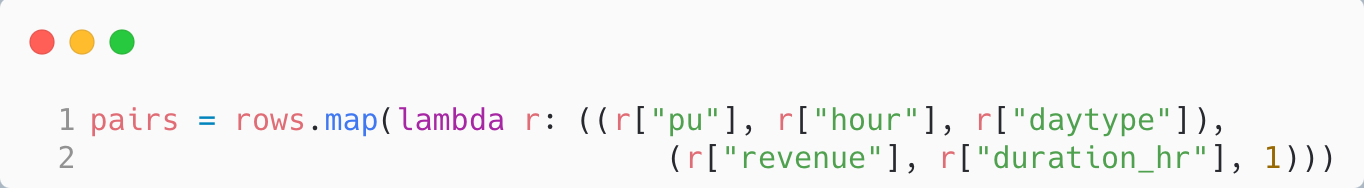
\includegraphics[width=1\linewidth]{Map.png}
    \caption{RDD formulation for mapping}
    \label{fig:mapping}
\end{figure}

\section{Shuffle / grouping}
xxx

\section{Reduction / aggregation}
xxx

\section{Spark execution and DAG}
xxx

\section{Results and technical interpretation}
xxx

\section{Visualisation}
xxx

\section{Business / societal interpretation and value}
xxx

\section{GitHub Repository}
The project setup and code can be found in the following GitHub repo: \url{https://github.com/ShreyaB143/MIT805-GroupProject}

\newpage
\clearpage 
\onecolumn 

\section{Appendix} 
xxx

\end{document}
